\documentclass{base}

\begin{document}

\cover
\newpage
\tableofcontents

\newpage
\begin{abstract}
	这里是摘要
\end{abstract}
\textbf{关键词}
\newpage

\section{绪论}
本次小学期要求制作的网站与数据库相结合的管理系统,基本要求是实现用户登录与数据库的增删查改。为了保证个人选题新颖的同时,又能满足所要求的技术栈,我选择了制作以经典电影《星际迷航》为主题的\textbf{星舰管理系统}。
\subsection{研究背景与研究意义}
《星际迷航》(\textit{Star Trek})是美国一部极具影响力的科幻电视系列剧,由吉恩·罗登贝瑞(Gene Roddenberry)创作。自 1966 年首次播出以来,这个系列已发展成为一个庞大的跨媒体特许经营,包括电视剧、电影、小说、漫画和电子游戏等。

影视中的星舰庞杂、类别繁琐,为该影视的爱好者实现一个星舰管理系统,\textbf{不仅能够建立起一个类星际迷航的维基百科式站点,也能锻炼学生的开发能力,让学生在兴趣中开发,从而不断激发其潜能。}
\subsection{设计内容}
本项目以星舰舰长的视角,设计了用户登录模块、星舰管理模块、武器管理模块、用户信息管理模块。各模块之间均有联系。
\subsection{课题研究方法}

为了实现星舰管理系统的开发,本次研究采用了文献综述法,通过查阅大量关于《星际迷航》的影视资料、书籍和相关论文,深入了解《星际迷航》的背景、星舰类型和特点。结合管理系统开发的相关技术文献,分析现有管理系统的设计模式和实现方法,为本课题提供理论支持。

通过问卷调查和访谈的形式,了解《星际迷航》爱好者对星舰管理系统的需求,明确系统的功能要求和用户体验需求。根据调查结果,确定系统的功能模块和设计框架。

采用SpringBoot和Vue技术栈进行系统的设计与开发。系统设计阶段包括模块划分、数据库设计和界面设计;开发阶段包括后端服务的实现、前端界面的开发及前后端的集成。

在系统开发完成后,通过单元测试、集成测试和用户测试等方式对系统进行全面测试,发现并修复系统中的缺陷。根据测试结果和用户反馈,对系统进行优化和迭代改进。

\subsubsection{技术路线与工具选择}


前端技术使用Vue.js,用于构建用户界面。Vue.js 是一款渐进式JavaScript框架,具有响应式的数据绑定和组件化开发的特点,非常适合构建复杂的单页面应用(SPA)。Vue Router用于管理前端路由,实现页面的导航和切换。Axios用于发送异步请求,与后端API进行数据交互。

\begin{figure}[H]
	\centering
	
\includegraphics[width=\linewidth]{images/vue-logo.png}
	\caption{Vue Logo}
	\label{fig:}
\end{figure}

后端技术使用Spring Boot,用于构建后端服务。Spring Boot 提供了开箱即用的配置和内嵌的服务器,使得开发、测试和部署变得更加简便。JPA (Java Persistence API):用于数据持久化操作,简化与数据库的交互。

\begin{figure}[H]
	\centering
	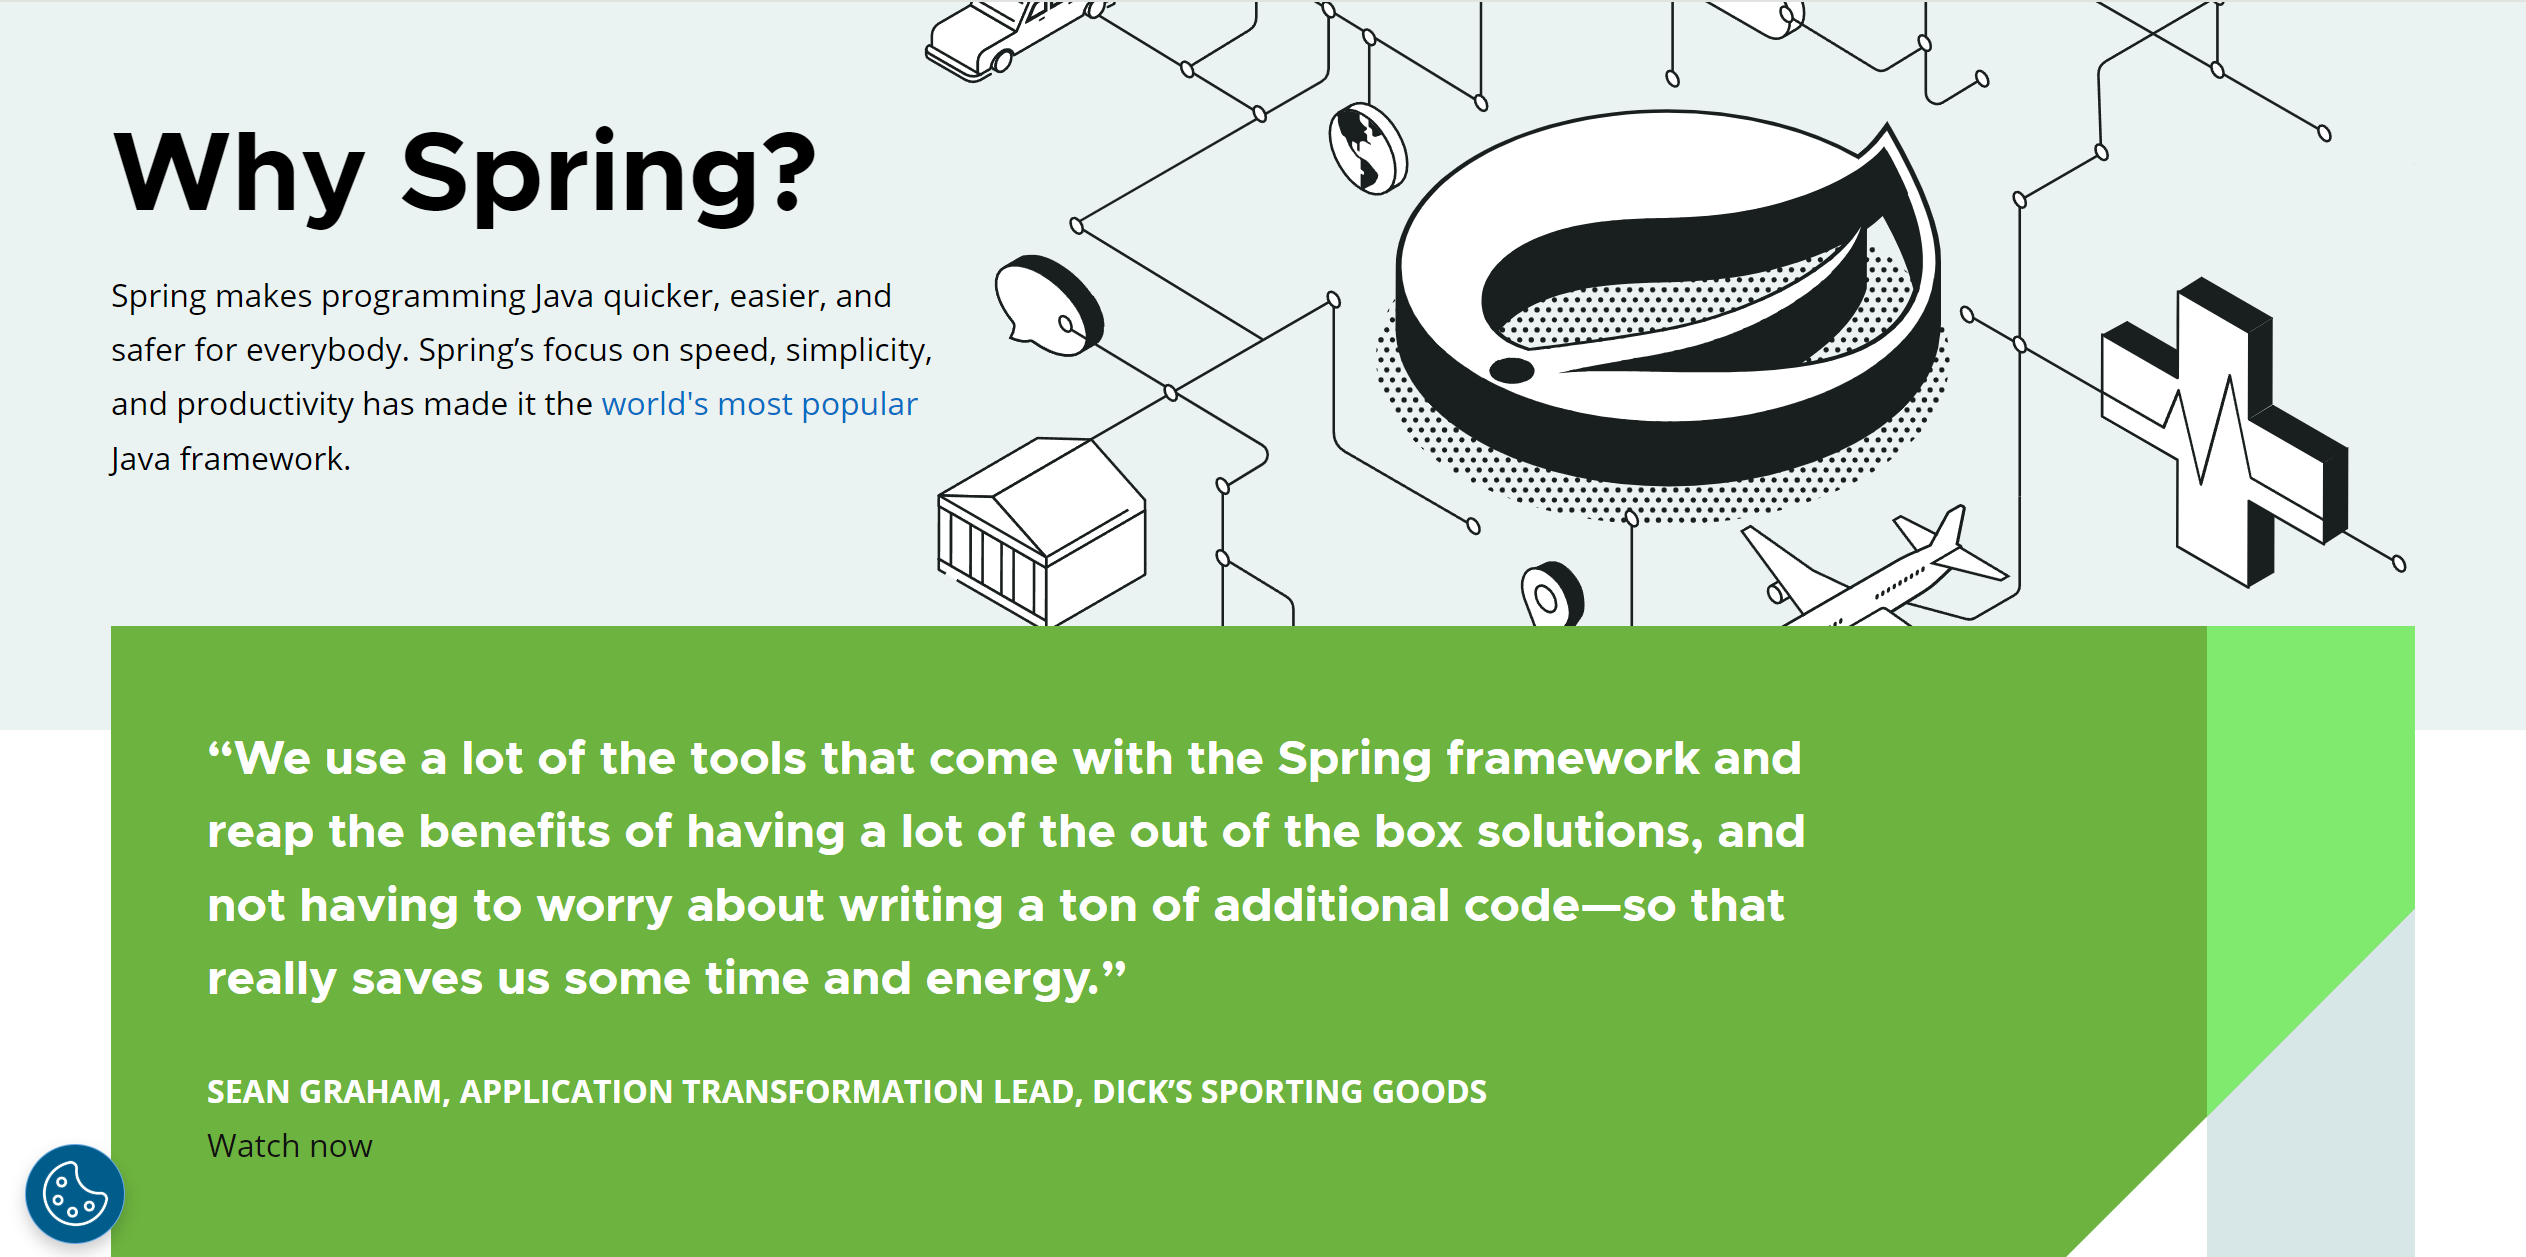
\includegraphics[width=\linewidth]{images/spring-web.png}
	\caption{Spring Boot 网站首页}
	\label{fig:}
\end{figure}

数据库使用MySQL,作为关系型数据库,用于存储用户信息、星舰数据和武器数据。MySQL 具有高性能、稳定性好、使用方便等特点。

开发工具使用IDEA,用于前后端代码的开发和调试,支持Spring Boot项目的快速创建和配置。

测试时,Postman用于测试后端API,验证接口的正确性和性能。Postman是一款用于API开发、测试和调试的工具。它提供了一个直观的界面,用户可以轻松地发送HTTP请求、查看响应、组织API文档和测试API功能。Postman支持多种协议,如HTTP、HTTPS、WebSocket等,是开发者在进行API开发和测试时的重要工具。

\begin{figure}[H]
	\centering
	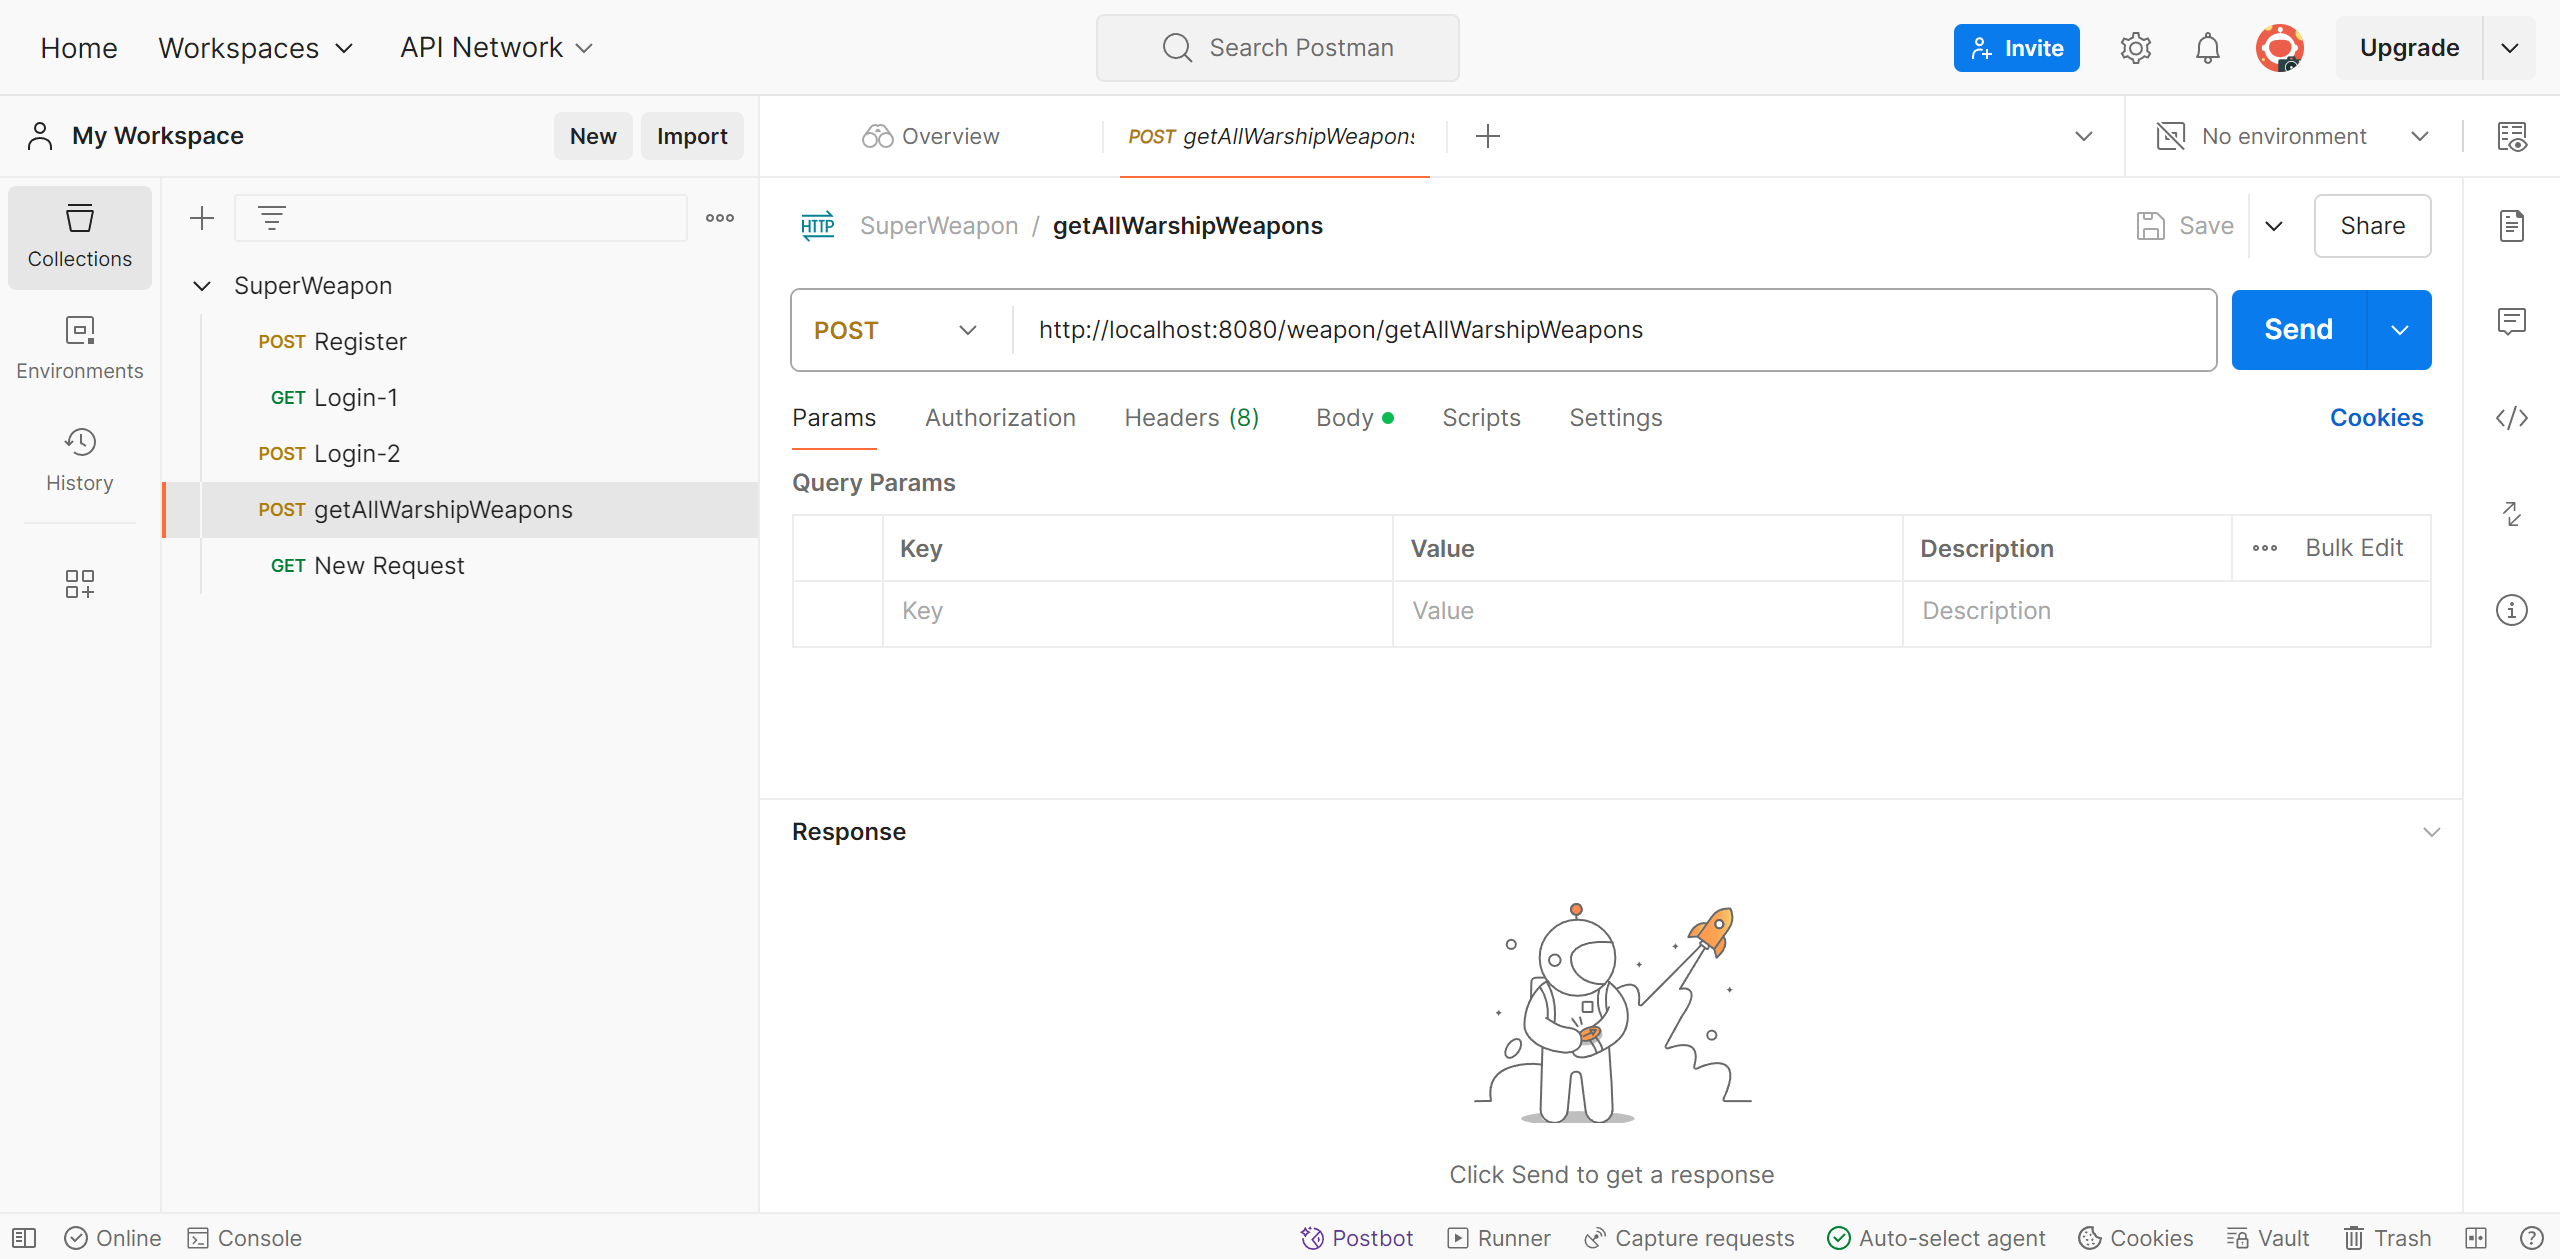
\includegraphics[width=\linewidth]{images/postman.png}
	\caption{后端开发时,正在使用 Postman 进行测试}
	\label{fig:}
\end{figure}

版本管理则使用Git用于版本控制,方便代码的管理。

\subsubsection{开发环境与测试环境搭建}

本次开发需要安装的开发工具有 IDEA ,可通过访问 \url{https://www.jetbrains.com/idea/} 下载。

剩下的环境我们使用 Chocolatey 进行安装,它是一个Windows上的软件包管理器,可以通过命令行轻松安装、更新和管理软件包。

以管理员身份打开 PowerShell ,然后执行:
\begin{verbatim}
	Set-ExecutionPolicy Bypass -Scope Process -Force;
	
	[System.Net.ServicePointManager]::SecurityProtocol = 
	[System.Net.ServicePointManager]::SecurityProtocol -bor 3072; 
	
	iex ((New-Object System.Net.WebClient)
	.DownloadString('https://community.chocolatey.org/install.ps1'))
\end{verbatim}

随后的安装就很简单了,下面直接安装 node.js、mysql、maven、java JDK:
\begin{verbatim}
	choco install nodejs mysql maven jdk17
\end{verbatim}

\section{系统分析}

\subsection{系统可行性分析}

评估星舰管理系统在技术、经济和操作方面的可行性。

\subsubsection{技术可行性}

系统采用 SpringBoot 和 Vue 技术栈,这两者都是当前流行且成熟的技术。SpringBoot 作为后端框架,具有快速开发、配置简单、社区支持丰富等优点,能够高效地实现复杂的业务逻辑和数据管理。Vue 作为前端框架,具有轻量、高效、易于学习和使用的特点,能够实现响应式和动态的用户界面。

数据库采用 MySQL,MySQL 是一个开源的关系型数据库管理系统,具有高性能、高可靠性和易于使用的特点,适合用于本项目的数据存储和管理。

\subsubsection{经济可行性}
系统开发所需的技术和工具(如 SpringBoot、Vue、MySQL 等)都是开源且免费的,这大大降低了开发成本。项目的开发团队主要由学生组成,不需要额外的人工成本。系统的部署可以选择免费的云服务器,进一步降低运行成本。

\subsubsection{操作可行性}
系统的用户主要为《星际迷航》的爱好者和开发团队成员。用户界面设计友好、易于操作,通过简单的注册和登录即可使用系统的各项功能。开发团队通过学习和实践,能够熟练掌握所需的技术和工具,确保项目的顺利进行。

\subsection{需求分析}

明确系统的功能需求和用户需求,为系统设计和开发提供依据。

\subsubsection{功能需求}
用户登录与注册,提供用户注册和登录功能,确保系统的安全性和个性化服务。
星舰管理,实现对星舰信息的增删查改,包括星舰名称、型号、所属舰队等信息。
武器管理,实现对星舰武器的增删查改,包括武器名称、类型、威力等信息。
用户信息管理,实现对用户信息的管理,包括用户名、邮箱、兴趣爱好等。
\subsubsection{用户需求}
便捷的操作界面,用户界面设计应简洁、美观,操作流程应简便,减少用户学习成本。
详细的星舰信息,提供详尽的星舰信息,包括历史背景、技术参数、服役情况等。
个性化服务,根据用户兴趣推荐相关的星舰和武器信息,提高用户体验。

\subsection{功能性要求}

功能性要求是对系统功能的详细描述,明确每个功能模块的具体实现。

\subsubsection{用户登录与注册模块}
\textbf{用户注册} 用户提供用户名、密码、邮箱等信息进行注册,注册信息保存到数据库。

\textbf{用户登录} 用户输入用户名和密码进行登录,系统验证用户信息,成功登录后进入系统主界面。

\subsubsection{星舰管理模块}

\textbf{新增星舰} 可以新增星舰信息,填写星舰名称、型号、所属舰队等。

\textbf{修改星舰} 可以修改已存在的星舰信息。

\textbf{删除星舰} 可以删除不再需要的星舰信息。

\textbf{查看星舰} 可以查看星舰的详细信息。

\subsubsection{武器管理模块}
\textbf{新增武器} 管理员可以新增武器信息,填写武器名称、类型、威力等。

\textbf{修改武器} 管理员可以修改已存在的武器信息。

\textbf{删除武器} 管理员可以删除不再需要的武器信息。

\textbf{查看武器} 所有用户都可以查看武器的详细信息。

\subsubsection{用户信息管理模块}

\textbf{修改用户信息} 用户可以修改自己的个人信息,包括用户名、邮箱、兴趣爱好等。
\textbf{查看用户信息} 用户可以查看自己的个人信息和系统中其他用户的公开信息。

\subsection{非功能性要求}

对系统性能、可靠性、安全性等方面的要求,确保系统的整体质量。

\subsubsection{性能要求}
系统响应时间应在合理范围内,用户操作后的响应时间不超过3秒。系统应能支持并发用户访问,至少支持1000个用户同时在线。

\subsubsection{可靠性要求}

系统应具有较高的稳定性,运行过程中无重大故障,月故障时间不超过1小时。系统应具有数据备份功能,防止数据丢失。

\subsubsection{安全性要求}
用户密码应加密存储,确保用户信息安全。系统应具有防护措施,防止SQL注入、跨站脚本等常见安全攻击。

\subsubsection{可维护性要求}
系统代码应具有良好的注释和文档,便于后续维护和升级。系统应具有日志记录功能,记录用户操作和系统运行情况,便于问题排查和解决。

\section{总体/概要设计}

星舰管理系统以模块化设计为核心,主要包括用户登录与注册模块、星舰管理模块、武器管理模块和用户信息管理模块。

\subsection{系统的功能模块}

\subsubsection{用户登录与注册模块}
\textbf{用户注册} 用户提供用户名、密码信息进行注册。
系统验证注册信息的有效性(例如用户名是否已存在、用户名格式是否正确等),验证通过后,将用户信息存储到数据库中。

\textbf{用户登录} 用户输入用户名和密码进行登录。系统验证用户信息是否正确,若正确则允许用户登录,进入系统主界面。若登录失败,提供相应的错误提示(例如用户名或密码错误)。

\textbf{用户注销} 用户可以选择注销当前登录状态,退出系统。

\subsubsection{星舰管理模块}

\textbf{新增星舰} 用户可以新增星舰信息,包括星舰名称、型号、所属舰队、建造时间等详细信息。系统对新增的星舰信息进行验证,并将其存储到数据库中。

\textbf{修改星舰} 用户可以修改已存在的星舰信息。系统对修改后的星舰信息进行验证,并更新数据库中的信息。

\textbf{删除星舰} 管理员可以删除不再需要的星舰信息。系统从数据库中删除对应的星舰记录。

\textbf{查看星舰} 用户可以查看星舰的详细信息,包括基本信息、历史背景、技术参数等。

\subsubsection{武器管理模块}

\textbf{新增武器} 可以新增武器信息,包括武器名称、类型、威力、装备星舰等详细信息。系统对新增的武器信息进行验证,并将其存储到数据库中。

\textbf{修改武器} 可以修改已存在的武器信息。系统对修改后的武器信息进行验证,并更新数据库中的信息。

\textbf{删除武器} 可以删除不再需要的武器信息。系统从数据库中删除对应的武器记录。

\textbf{查看武器} 可以查看武器的详细信息,包括基本信息、技术参数、装备星舰等。

\subsubsection{用户信息管理模块}
\textbf{查看用户信息} 用户可以查看自己的个人信息,包括用户名、邮箱、兴趣爱好等。用户可以查看系统中其他用户的公开信息(如用户名、兴趣爱好等)。

\textbf{修改用户信息} 用户可以修改自己的个人信息,包括用户名、邮箱、兴趣爱好等。系统对修改后的用户信息进行验证,并更新数据库中的信息。

\subsection{各个模块之间的主要关系}

\subsection{数据库设计}

\subsubsection{数据模型与数据结构}

\subsubsection{数据存储与访问策略}

\section{详细设计}

\section{系统测试}

\section{存在的问题与总结}

\subsection{存在的问题}

\subsection{总结}

星舰管理系统的开发项目以经典电影《星际迷航》为主题,为《星际迷航》爱好者提供一个管理和查询星舰信息的平台。本项目采用SpringBoot和Vue技术栈,设计并实现了用户登录与注册、星舰管理、武器管理和用户信息管理等功能模块。

在开发过程中,通过文献综述法和问卷调查法,充分了解了《星际迷航》的背景和用户需求,为系统的设计和实现提供了理论支持和实践依据。尽管在技术集成、需求变更、数据安全和用户体验等方面存在一些挑战,但通过合理的设计和有效的管理,系统可以满足预期的功能和性能要求。

未来,系统可以根据用户的反馈和需求不断进行功能扩展和性能优化,以提供更好的用户体验和更丰富的功能。开发团队需要继续关注技术的发展和用户需求的变化,保持系统的先进性和实用性。

通过本次项目的开发,我够在实践中提升开发技能,掌握SpringBoot和Vue等技术的应用,还能够在项目管理、团队协作和问题解决等方面得到锻炼,为未来的学习和工作打下坚实的基础。

\end{document}